\documentclass[aspectratio=169,10pt]{beamer}
\usepackage{graphicx}
\usepackage{booktabs}
\usepackage{array}
\usepackage{amsmath}
\graphicspath{{../figures/sigma0/}}

%-- red colour theme (as update_talk_2026-10.tex) --
\definecolor{ubred}{RGB}{160,20,20}
\definecolor{ubdark}{RGB}{90,10,10}
\definecolor{ublight}{RGB}{205,70,70}
\usetheme{default}
\usecolortheme{default}
\setbeamercolor{structure}{fg=ubred}
\setbeamercolor{title}{fg=ubdark}
\setbeamercolor{frametitle}{fg=white,bg=ubred}
\setbeamercolor{section in head/foot}{fg=white,bg=ubdark}
\setbeamercolor{alerted text}{fg=ubred}
\setbeamercolor{block title}{fg=white,bg=ubred}
\setbeamercolor{block body}{bg=ubred!8}
\setbeamercolor{itemize item}{fg=ubred}
\setbeamercolor{itemize subitem}{fg=ublight}
\setbeamertemplate{navigation symbols}{}
\setbeamertemplate{frametitle}{\vskip4pt\usebeamercolor[fg]{frametitle}%
  \begin{beamercolorbox}[wd=\paperwidth,ht=2.4ex,dp=1ex,leftskip=.3cm]{frametitle}%
  \bfseries\insertframetitle\end{beamercolorbox}}
\newif\ifbackup
\setbeamertemplate{footline}{%
  \leavevmode\hbox{%
  \begin{beamercolorbox}[wd=.62\paperwidth,ht=2.4ex,dp=1ex,leftskip=.3cm]{section in head/foot}%
  \usebeamerfont{author in head/foot}\insertshortauthor\ | MicroBooNE NuMI $\Sigma^0$\hfill\end{beamercolorbox}%
  \begin{beamercolorbox}[wd=.38\paperwidth,ht=2.4ex,dp=1ex,rightskip=.3cm]{section in head/foot}%
  \hfill\insertshorttitle\quad\ifbackup Backup \insertframenumber\else\insertframenumber\,/\,\pageref{mainend}\fi\end{beamercolorbox}}}

\newcommand{\Szero}{\ensuremath{\Sigma^{0}}}
\newcommand{\Lam}{\ensuremath{\Lambda}}
\newcommand{\numubar}{\ensuremath{\bar{\nu}_\mu}}
\newcommand{\muUL}{\ensuremath{\mu_{\mathrm{UL}}}}

\title[$\Sigma^0$ status]{Search for $\Sigma^0$ production in $\bar\nu_\mu$ charged-current interactions in the NuMI beam}
\subtitle{Two selections and the expected sensitivity}
\author[Nowak, Patel]{J.~Nowak and N.~Patel}
\date{October 2026}

\begin{document}

{\setbeamertemplate{footline}{}
\begin{frame}[plain]
  \titlepage
  \begin{center}\small\color{ubdark}
  $\bar\nu_\mu\,\mathrm{Ar}\to\mu^+\Sigma^0X$, \;$\Sigma^0\to\Lambda\gamma$, \;$\Lambda\to p\pi^-$
  \;$\bullet$\; RHC, $1.15\times10^{21}$~POT \;$\bullet$\; signal region blind\\[3pt]
  \footnotesize Details: \texttt{report/other\_notes/sigma0\_note.pdf}
  \end{center}
\end{frame}}

% ---------------------------------------------------------------------------
\begin{frame}{Summary}
  \begin{itemize}
    \item Two independent selections:
      \begin{itemize}
        \item \textbf{PeLEE BDT}: standard PeLEE ntuples, cross-validated gradient BDT.
              Has data, EXT and dirt. $S=2.11$ / $13.1$ (NuWro / GENIE), $B=382$.
        \item \textbf{\Lam-style}: HyperonProduction ntuples, fitted \Lam\ decay vertex and a
              wire-level ``island'' test. $S=0.142$ / $1.01$, $B=4.4$: $6\times$ the
              purity, $1/15$ of the signal. No data or dirt in that format.
      \end{itemize}
    \item \textbf{The result will be an upper limit.} Median discovery significance at the
          predicted rate: $\leq0.6\sigma$.
    \item Best median expected 90\%~CL limit: \alert{$\sim3\times$ the GENIE rate,
          $\sim18\times$ the NuWro rate}. The generators differ by $6\times$: NuWro has
          hyperon FSI, GENIE does not.
    \item Under one signal model the \textbf{PeLEE chain gives the better limit below a
          $\sim20\%$ background systematic}, and the two are within $10\%$ up to $30\%$.
          Purity alone pointed the other way.
    \item Next: the \alert{background systematics of the PeLEE chain}, which set the limit.
  \end{itemize}
\end{frame}

% ===========================================================================
\section{Signal and samples}

\begin{frame}{The signal}
  \begin{columns}[T]
  \column{0.52\textwidth}
  \small
  \begin{itemize}
    \item $\bar\nu_\mu$ CC, a \Szero\ in the final state, true vertex in the FV.
    \item $\Szero\to\Lam\gamma$ ($\sim100\%$): soft photon,
          $E_\gamma = 74.5$~MeV in the rest frame.
    \item $\Lam\to p\pi^-$ ($63.9\%$): the \Lam\ is slow ($\beta\gamma\approx0.4$), flight
          median $1.85$~cm, mean $3.2$~cm.
    \item Primary-vertex resolution $5.5$~cm: the flight cannot be measured from the
          Pandora vertex ($r=-0.014$), but the decay topology can be tested at wire level.
    \item Reconstruction ceiling: all four particles found in $18\%$ of signal; the
          $\pi^-$ in $47\%$.
  \end{itemize}
  \column{0.45\textwidth}
  \footnotesize
  \textbf{In-FV \Szero\ per $1.15\times10^{21}$~POT}\\[2pt]
  \begin{tabular}{lr}
    \toprule
    GENIE overlay (no hyperon FSI) & 83.3 \\
    GENIE hyperon sample & 110.1 \\
    NuWro run3b, flux-weighted & 12.8 \\
    \bottomrule
  \end{tabular}\\[4pt]
  NuWro/GENIE $=0.15$: hyperon FSI $4.19\times$, old flux $1.48\times$, production
  $1.05\times$; product $6.51\times$ = measured. A NuWro CCQE control run agrees with
  GENIE's rate to $17\%$.\\[4pt]
  \alert{A model choice, not a bug}: every result is quoted under both.
  \end{columns}
\end{frame}

\begin{frame}{Samples}
  \footnotesize
  \begin{tabular}{llp{0.55\textwidth}r}
    \toprule
    format & sample & content & scale \\
    \midrule
    PeLEE & \Szero\ signal & NuWro run3b overlay (local production), 250k events, flux-weighted & $8.6\times10^{-4}$ \\
          & $\nu$ background & RHC overlay Runs 1, 2, 3, 4a, 4b, 4c, $1.55\times10^{22}$~POT & $0.075$ \\
          & dirt & RHC Runs 1, 2b, 3b, 4a, 4b, $1.74\times10^{21}$~POT, old flux & $0.66$ \\
          & EXT & run3b beam-off, $3.27\times10^{7}$ gates & $0.75$ \\
    \midrule
    hypana & \Szero\ signal & GENIE hyperon sample; NuWro run3b & \\
           & $\nu$ background & 14\,164 files, $7.05\times10^{21}$~POT & $0.16$ \\
           & EXT & 16\,570 events (local reco2 $+$ HyperonProduction) & $150$ \\
           & dirt, data & --- & \\
    \bottomrule
  \end{tabular}\\[6pt]
  \textbf{Fixed in the PeLEE background (17 October):}
  \begin{itemize}
    \item the dirt was FHC ($\langle E_\nu\rangle$ and spectra), now RHC; it is on the old NuMI flux and takes the NuWro flux map;
    \item the Run~3 overlay was missing ($+55\%$ background statistics);
    \item EXT added; GENIE \Szero\ inside the overlay no longer counted as background.
  \end{itemize}
\end{frame}

% ===========================================================================
\section{PeLEE chain}

\begin{frame}{PeLEE chain: selection and BDT}
  \begin{columns}[T]
  \column{0.46\textwidth}
  \small
  \begin{itemize}
    \item Cosmic veto (topological score $>0.2$), $1$--$3$ showers, muon candidate,
          $<5$ tracks.
    \item Proton and pion: best \emph{ordered pair} from a joint per-role score; pion
          purity $33.5\to42.5\%$ (ceiling $51\%$). Formed when present, \emph{not
          required}: requiring them halved the figure of merit.
    \item 57 BDT inputs: PID, distances, angles, \Lam\ and \Szero\ masses, pointing,
          $\pi^0$ and second-shower variables, \texttt{HasPair}.
    \item Two-fold cross-validation by event parity: every score is out of sample.
    \item \textbf{Retrained 18 Oct}: EXT in the background tree ($+5\%$), and training
          on $95\%$ of each fold, not TMVA's default $50\%$ ($+4\%$). AUC
          $0.889\to0.900$.
  \end{itemize}
  \column{0.52\textwidth}
  \centering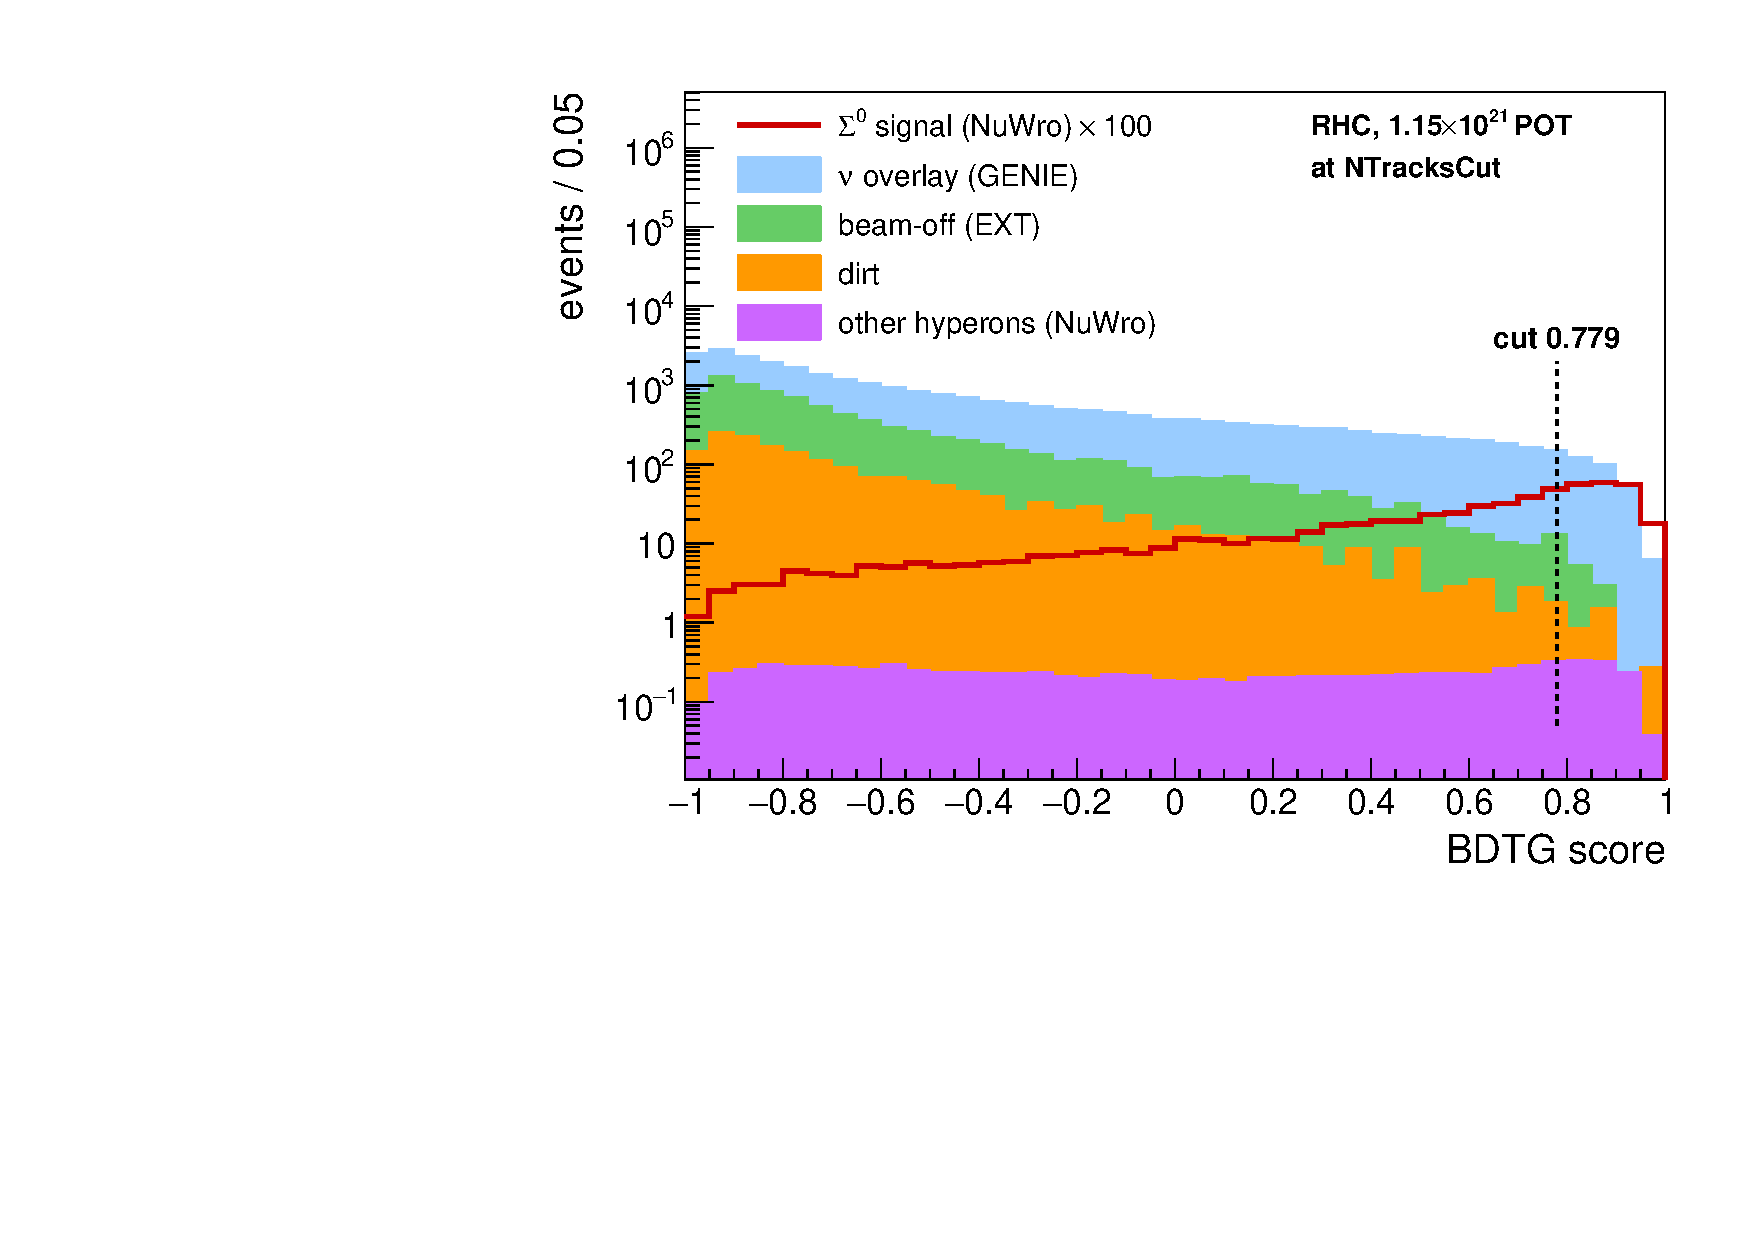
\includegraphics[width=\textwidth]{bdt_score}\\
  \footnotesize cross-validated BDTG score at preselection
  \end{columns}
\end{frame}

\begin{frame}{PeLEE chain: results at BDTG $>0.759$}
  \begin{columns}[T]
  \column{0.55\textwidth}
  \footnotesize
  \begin{tabular}{lrrrr}
    \toprule
    stage & raw sig. & eff. & $S$ & $B$ \\
    \midrule
    MuonCandidate & 11107 & $51.6\%$ & 6.47 & 28978 \\
    NTracksCut    & 10931 & $50.8\%$ & 6.37 & 26549 \\
    \textbf{BDTG} & \textbf{3644} & $\mathbf{16.9\%}$ & \textbf{2.11} & \textbf{382} \\
    \bottomrule
  \end{tabular}\\[6pt]
  \begin{tabular}{lrrr}
    \toprule
    $B$ at BDTG & old BDT (0.616) & new (0.759) & raw \\
    \midrule
    overlay & 715.7 & 367.9 & 5178 \\
    EXT     & 109.5 & 11.3  & 15 \\
    dirt    & 13.8  & 2.3   & 7 \\
    other hyperons & 1.7 & 1.1 & 1841 \\
    \midrule
    total   & 840.7 & \textbf{382.4} & \\
    \bottomrule
  \end{tabular}\\[4pt]
  purity $0.34\%\to\mathbf{0.55\%}$, \;$S/\sqrt{S+B}$ $0.098\to\mathbf{0.108}$
  \column{0.42\textwidth}
  \small
  \textbf{GENIE signal through the same chain}\\
  The overlay's own \Szero\ (never trained on):\\
  $S_{\mathrm{GENIE}}=13.1\pm1.0$ (187 raw), efficiency $18.0\%$ against NuWro's
  $16.8\%$.\\[2pt]
  $\Rightarrow$ the limit on the number of events is model-independent to a few \%.\\[8pt]
  \textbf{Detector variations} (Run~3 set, 9 variations)\\
  None resolved: quadrature $5.2\%$ on $B$ (MC noise $6.8\%$), $21.7\%$ on $S$ (noise
  $21.1\%$).\\
  $\Rightarrow$ $\lesssim7\%$ on $B$; not measured on $S$.
  \end{columns}
\end{frame}

% ===========================================================================
\section{Lambda-style chain}

\begin{frame}{\Lam-style chain: following the \Lam\ CCQE analysis}
  \begin{columns}[T]
  \column{0.33\textwidth}
  \footnotesize
  \begin{itemize}
    \item The \Lam\ CCQE analysis reaches $91\%$ purity; at equal efficiency our earlier
          hypana BDT had $2.8\%$.
    \item Score every ordered track pair; pair precuts are a preference, not a veto.
    \item Fit the decay vertex (V fit): decay length, pointing angle $\alpha$.
    \item \textbf{Island test}: grow clusters of raw wire activity from the $\mu$, $p$ and
          $\pi$ starts; require $p$ and $\pi$ to merge and the $\mu$ to stay apart, on
          $\geq2$ planes.
    \item Needs wire windows: hypana format only.
  \end{itemize}
  \column{0.66\textwidth}
  \centering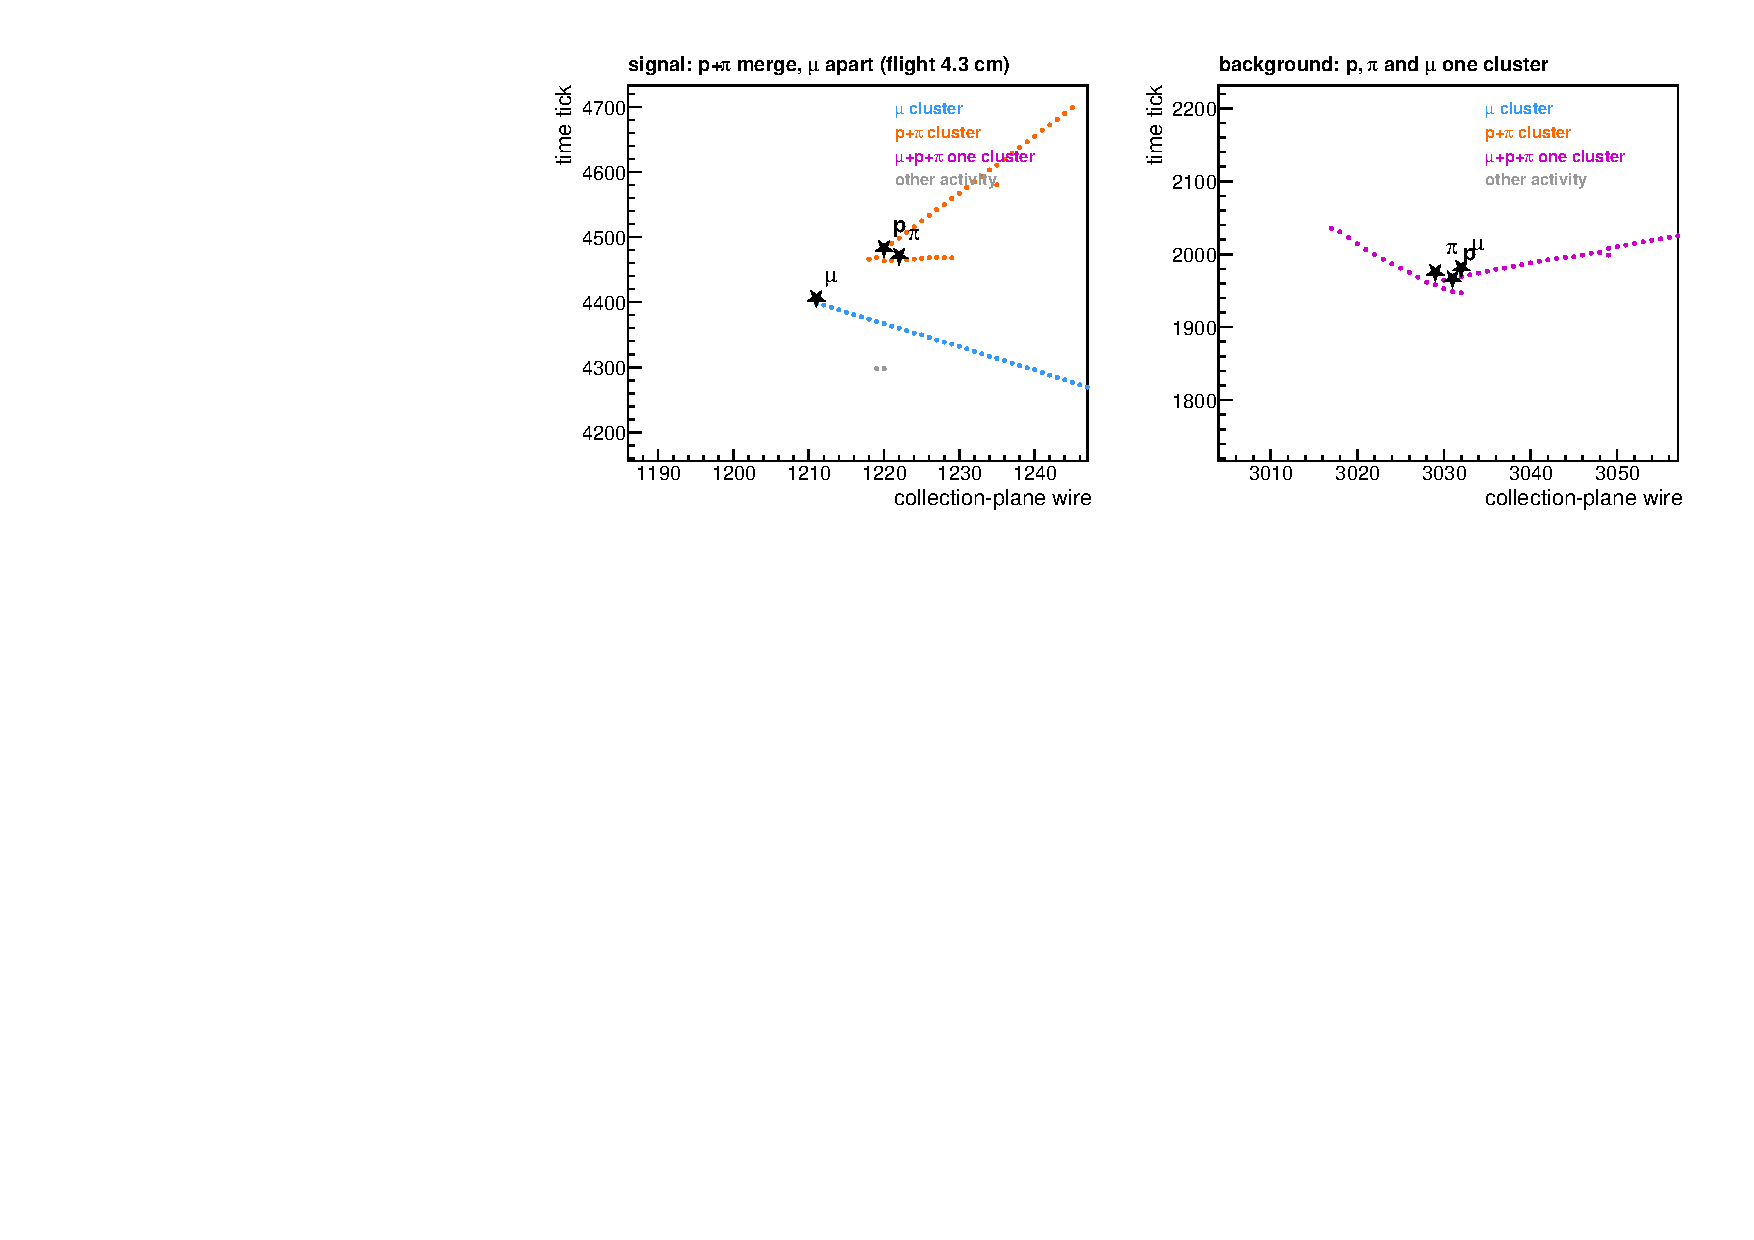
\includegraphics[width=\textwidth]{island_display}\\
  \footnotesize collection plane; left: signal with $4.3$~cm flight, right: background
  \end{columns}
\end{frame}

\begin{frame}{\Lam-style chain: operating point}
  \begin{columns}[T]
  \column{0.55\textwidth}
  \footnotesize\setlength{\tabcolsep}{3.5pt}
  \begin{tabular}{lrrrr}
    \toprule
    stage & raw sig & raw bkg & $S$ (GENIE) & $B$ \\
    \midrule
    MuonCandidate & 3043 & 123000 & 58.7 & 20113 \\
    pair          &  921 &  51238 & 17.8 &  8378 \\
    $m_{p\pi}$ $\pm20$~MeV & 504 & 16391 & 9.72 & 2680 \\
    pointing      &  144 &    706 & 2.78 & 115.4 \\
    photon gap $>2$~cm & 139 & 549 & 2.68 & 89.8 \\
    \textbf{island, $\geq2$ planes} & \textbf{69} & \textbf{23} & $\mathbf{1.33}$ & $\mathbf{3.76}$ \\
    \bottomrule
  \end{tabular}\\[4pt]
  $+$ EXT $0.62\pm0.27$ $+$ NuWro FSI $0.02$ $\Rightarrow$ $B=4.40$, purity $23\%$.\\
  NuWro: $S=0.142$ (245 raw), efficiency $0.42\%$ vs $0.46\%$.\\[4pt]
  \textbf{Island pass rate vs true flight}\\
  \begin{tabular}{lrrrr}
    \toprule
    flight & 1--2 & 2--3 & 3--5 & 5--10 cm \\
    \midrule
    connectivity $3\times40$ & 19\% & 45\% & 70\% & 86\% \\
    $2\times20$ (now)        & 43\% & 80\% & 85\% & 91\% \\
    \bottomrule
  \end{tabular}
  \column{0.41\textwidth}
  \centering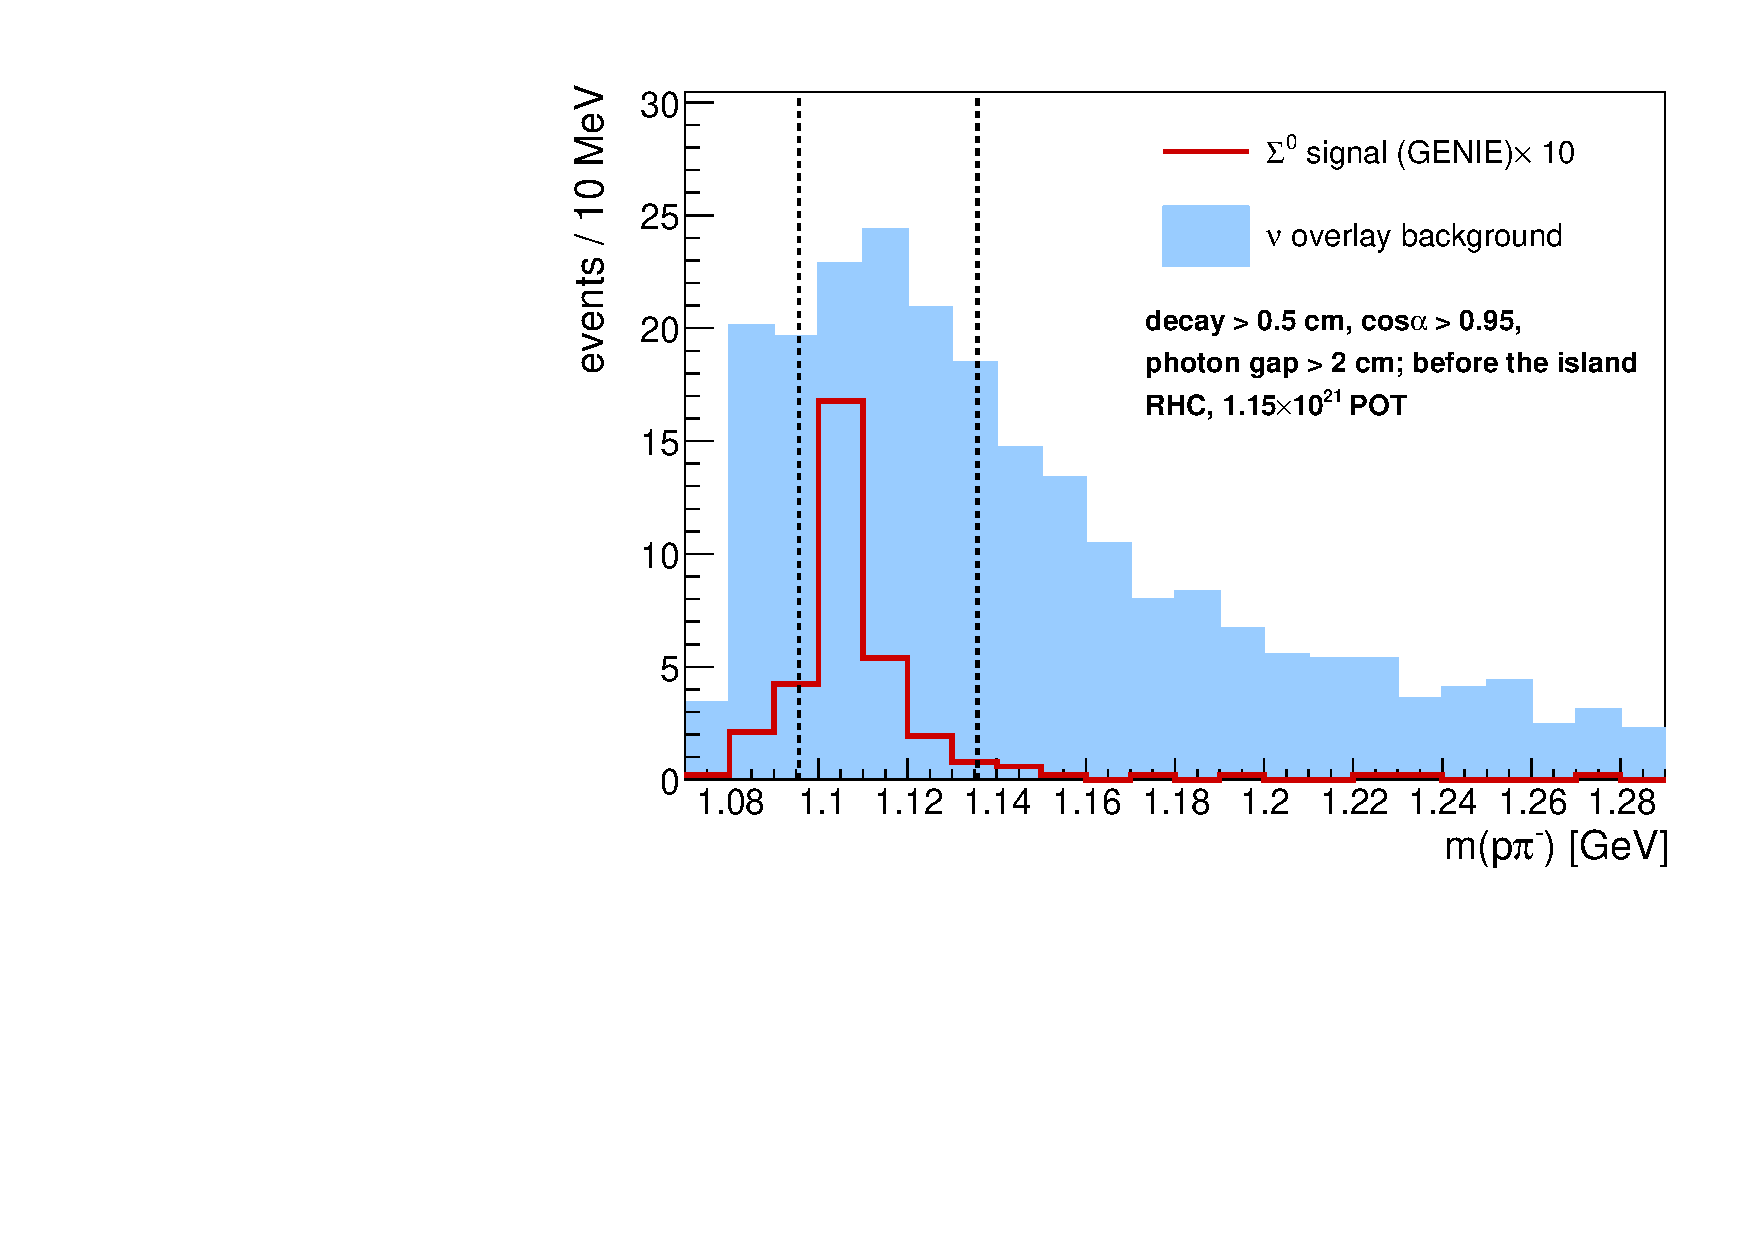
\includegraphics[width=\textwidth]{lambda_mass}\\
  \footnotesize before the mass window and the island test\\[2pt]
  \raggedright
  Out of sample: the photon gap, fixed in September on the Run~3 list, halves the
  background of the independent extension at $96\%$ signal efficiency.
  \end{columns}
\end{frame}

\begin{frame}{\Lam-style chain: beam-off background}
  \small
  \begin{itemize}
    \item 3\,349 run3b \texttt{ext\_unbiased} files through reco2 and HyperonProduction
          locally: 16\,570 events, $150$ data events each. Too few to reach the
          operating point (0 of 76 pass the pointing cut).
    \item Factorised: EXT at MuonCandidate $\times$ pass fraction of the overlay's own
          cosmic-dominated candidates.
  \end{itemize}
  \footnotesize
  \begin{center}
  \begin{tabular}{lrrrrr}
    \toprule
    step & EXT raw & EXT $P$ & cosmic MC raw & cosmic MC $P$ & all-bkg $P$ \\
    \midrule
    MuonCandidate & 76 & -- & 4\,220 & -- & -- \\
    pair & 8 & $0.105\pm0.035$ & 571 & $0.135\pm0.005$ & 0.42 \\
    $m_{p\pi}$ window & 3 & $0.38\pm0.17$ & 165 & $0.289\pm0.019$ & 0.32 \\
    pointing & 0 & 0 of 3 & 7 & $0.042\pm0.016$ & 0.043 \\
    \bottomrule
  \end{tabular}
  \end{center}
  \small
  \begin{itemize}
    \item \textbf{EXT $=0.62\pm0.27$}. Real cosmics confirm the factorisation where they
          have events: 8 of 76 pairs vs 10 from the cosmic MC, 32 from the neutrino rate.
    \item Open: the island and gap steps borrow the neutrino-background rate; without
          that, EXT $<6.2$ at 90\% CL.
  \end{itemize}
\end{frame}

% ===========================================================================
\section{Expected sensitivity}

\begin{frame}{Expected sensitivity: method}
  \small
  \begin{itemize}
    \item One-bin counting, $n\sim\mathrm{Pois}(\mu S e + b)$, with $\mu$ the \Szero\ rate in
          units of the model.
    \item $b$: lognormal, width $=$ MC statistics $\oplus$ background systematic $f$
          (scanned 0--30\%).
    \item $e$: lognormal, $20\%$ signal normalisation (placeholder) $\oplus$ signal MC
          statistics.
    \item Bayesian limit, flat prior in $\mu$, nuisances marginalised; hybrid CL$_s$ is
          $4\%$ tighter. Both reproduce the PDG table for a known background.
    \item Expected limit: at the median $n$ of $\mathrm{Pois}(B)$, band from the 16 and
          84\% quantiles.
    \item The PeLEE BDT cut is also re-chosen for each $f$ to minimise the limit.
    \item \texttt{Sigma/pelee/Sensitivity.C}
  \end{itemize}
  \vspace{4pt}
  \begin{block}{Both chains under one model}
  NuWro: PeLEE $S=2.11$, \Lam-style $S=0.142$. \quad GENIE (overlay normalisation): PeLEE
  $13.1$, \Lam-style $1.01$.\\
  Under the same model, purity favours the \Lam-style chain $\sim6\times$ ($3.1\%$ vs $0.55\%$, NuWro)
  and signal yield favours the PeLEE chain $15\times$.
  \end{block}
\end{frame}

\begin{frame}{Expected sensitivity: result}
  \centering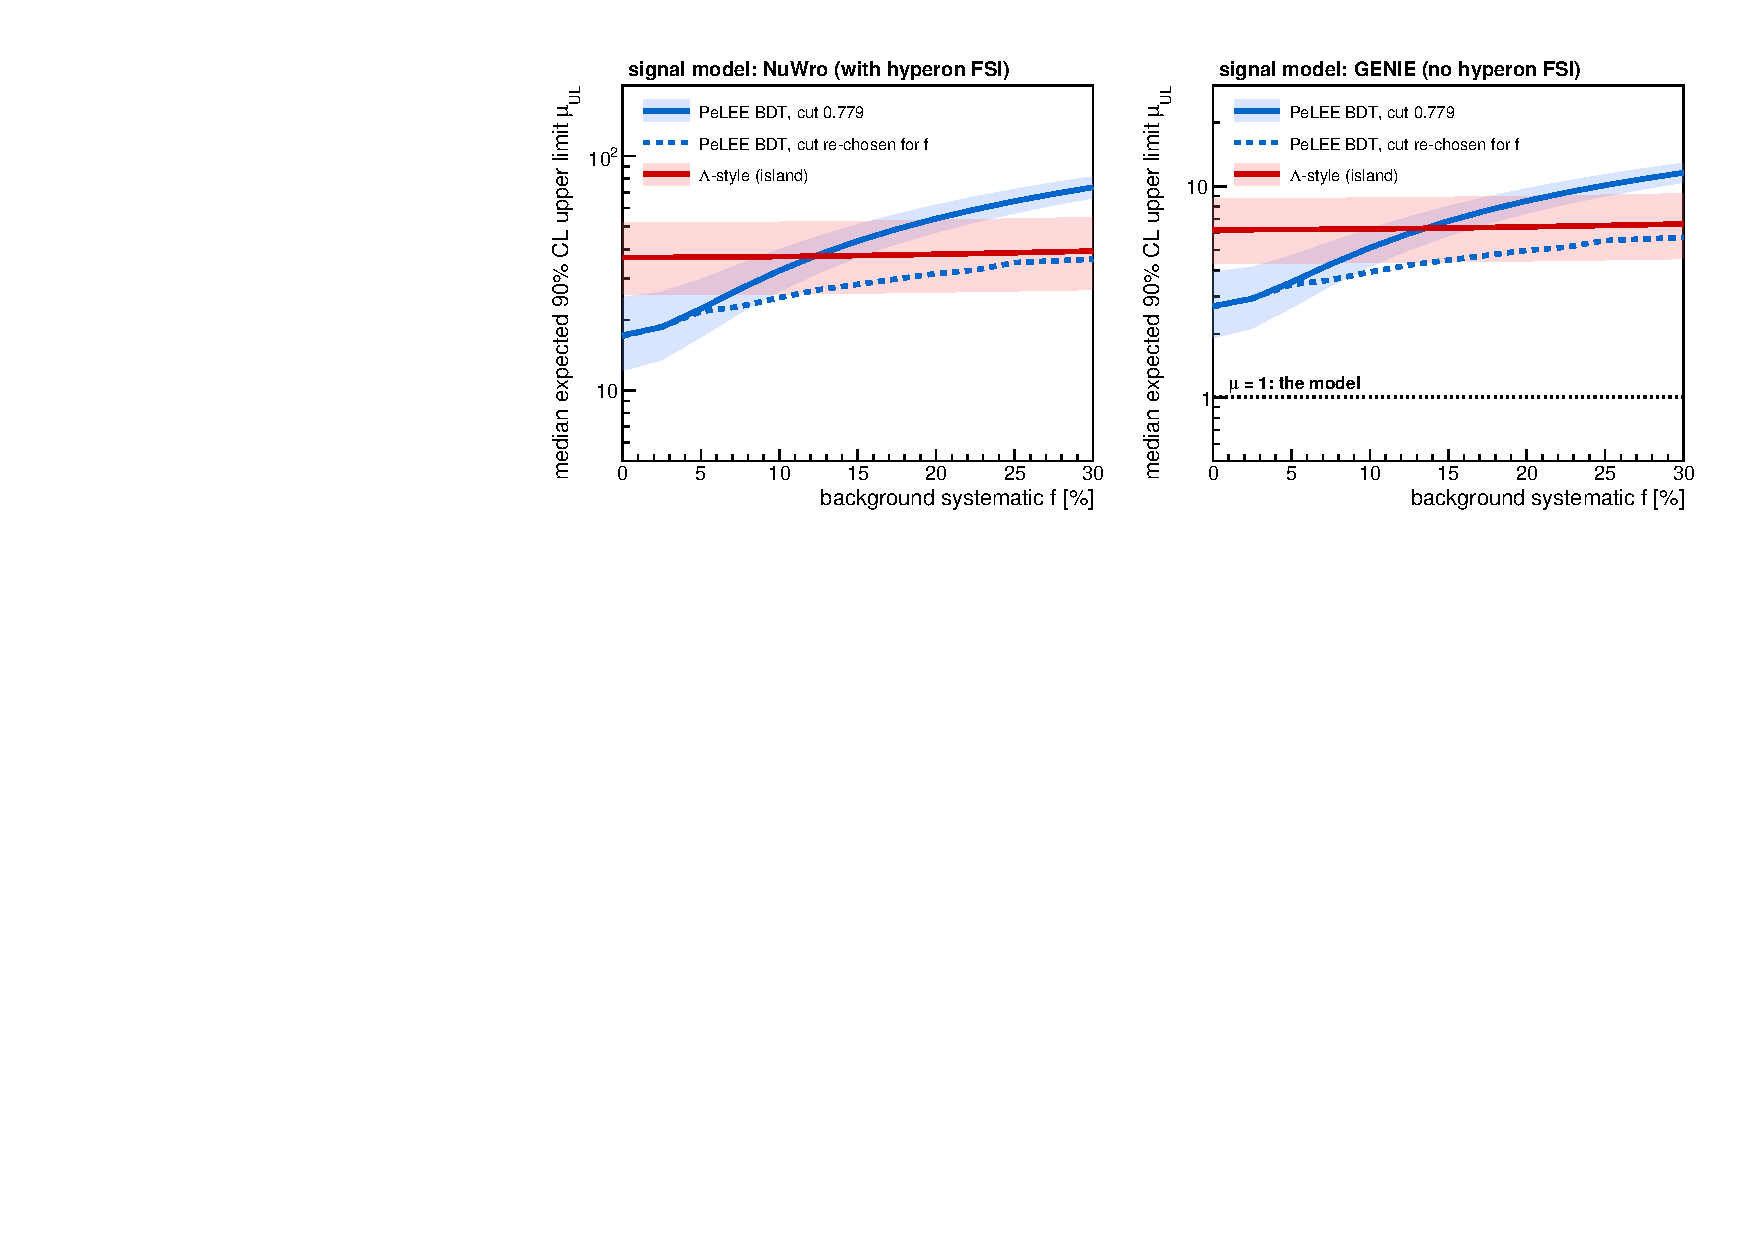
\includegraphics[width=0.86\textwidth]{limit_vs_f}\\[2pt]
  \footnotesize
  \begin{tabular}{lccc}
    \toprule
    median $\muUL$, NuWro / GENIE & $f=0$ & $f=15\%$ & $f=30\%$ \\
    \midrule
    PeLEE, cut 0.759        & 18.1 / 2.95 & 48.2 / 7.88 & 82.3 / 13.5 \\
    PeLEE, cut re-chosen    & 18.1 / 2.91 \;(0.750) & 31.0 / 5.00 \;(0.890) & 38.2 / 6.16 \;(0.925) \\
    \Lam-style              & 36.9 / 5.33 & 37.6 / 5.43 & 39.3 / 5.68 \\
    \bottomrule
  \end{tabular}
\end{frame}

\begin{frame}{What the sensitivity says}
  \begin{enumerate}
    \item \textbf{A limit, not an observation.} Best median $Z = 0.63\sigma$ (GENIE).
          The best limit is $\sim220$ in-FV \Szero\ events; GENIE predicts 73, NuWro 13.
    \item \textbf{The PeLEE chain is better below $f\approx20\%$}: $2.0\times$ at $f=0$,
          $1.4\times$ at $10\%$, $1.2\times$ at $15\%$ (NuWro). From 20 to 30\% the two are
          within $10\%$, and the model decides which is ahead.
    \item \textbf{The \Lam-style limit is set by Poisson counting} at $B\approx4.4$:
          perfect knowledge of $B$ moves it by $3\%$, dirt at its bound by at most $16\%$.
          Hypana data and dirt would give a cross-check with different systematics, not a
          better limit.
    \item \textbf{The background systematic drives the PeLEE limit}: $\times1.7$ from
          $f=0$ to $15\%$ even with the cut re-chosen.
    \item \textbf{Choose the BDT cut from the systematic budget}: at $f=10\%$, 0.875
          instead of 0.759 is $25\%$ better. $S/\sqrt{S+B+(fB)^2}$ agrees up to $10\%$ and
          then picks cuts with too few raw events.
  \end{enumerate}
\end{frame}

% ===========================================================================
\section{Next steps}

\begin{frame}{Next steps}
  \begin{enumerate}
    \item \textbf{Background systematics, PeLEE chain}: flux (\texttt{weightsPPFX}), cross
          section (\texttt{weightsGenie}) and reinteraction (\texttt{weightsReint})
          multisims at one bin -- the ntuples carry them, no framework port needed --
          plus detector variations ($\lesssim7\%$).
    \item \textbf{Constrain $B$ from data}: fit the low-BDT-score region, where the
          signal is negligible, and extrapolate; the $\pi^0$ normalisation is the target.
    \item \textbf{Set the BDT cut} from the resulting $f$; redo the detector variations
          there.
    \item \textbf{Signal model}: quote under NuWro and GENIE; understand the
          $1.3$--$1.6\times$ spread among the GENIE samples.
    \item \textbf{Closure}: Poisson-thrown fake data, with the overlay's GENIE \Szero\ as
          an injected alternative signal.
    \item \textbf{Unblind} the RHC beam-on PeLEE data and set the observed limit.
    \item Later: \Lam-style data and dirt as a cross-check; FHC$+$RHC.
  \end{enumerate}
  \label{mainend}
\end{frame}

% ===========================================================================
\backuptrue
\appendix
\section*{Backup}

{\setbeamertemplate{footline}{}
\begin{frame}[plain]
  \begin{center}\Huge\color{ubred} Backup\end{center}
\end{frame}}

\begin{frame}{Backup: BDT retraining, out of sample}
  \footnotesize
  \begin{center}
  \begin{tabular}{lcccccc}
    \toprule
    training & AUC & \multicolumn{3}{c}{$B/B_0$ at signal efficiency} & \multicolumn{2}{c}{peak $S/\sqrt{S+B}$} \\
             &     & $50\%$ & $40\%$ & $20\%$ & value & cut \\
    \midrule
    15 Oct (no EXT, half fold)  & 0.8894 & 0.0412 & 0.0253 & 0.0067 & 0.0993 & 0.690 \\
    EXT, half fold (3 seeds)    & 0.896 & 0.038 & 0.023 & 0.006 & 0.104--0.105 & \\
    \textbf{EXT, 95\% of fold}  & \textbf{0.9000} & \textbf{0.0358} & \textbf{0.0215} & \textbf{0.0061} & \textbf{0.1077} & \textbf{0.759} \\
    EXT, 95\% (2 other seeds)   & 0.900--0.902 & 0.035 & 0.021 & 0.006 & 0.108--0.109 & \\
    \bottomrule
  \end{tabular}
  \end{center}
  \small
  \begin{itemize}
    \item EXT in training: at $50\%$ signal efficiency $0.9\%$ of EXT survives against $2.2\%$;
          overlay unchanged.
    \item Full fold: every full-fold seed beats every half-fold seed; reseeding moves the
          figure of merit by $\pm0.5\%$. The BDT still gains from more signal.
    \item Default seed adopted, not the best one; \texttt{TrainBDT.C} reproduces it exactly.
  \end{itemize}
\end{frame}

\begin{frame}{Backup: detector variations at BDTG $>0.759$}
  \footnotesize
  \begin{columns}[T]
  \column{0.5\textwidth}
  \begin{tabular}{lrr}
    \toprule
    variation & $S$ var/CV & $B$ var/CV \\
    \midrule
    LY attenuation   & $1.000\pm0.000$ & $0.997\pm0.005$ \\
    LY down          & $0.975\pm0.025$ & $0.985\pm0.006$ \\
    LY Rayleigh      & $0.980\pm0.039$ & $0.987\pm0.008$ \\
    recombination    & $1.062\pm0.088$ & $0.973\pm0.030$ \\
    SCE              & $0.921\pm0.090$ & $0.998\pm0.034$ \\
    WireMod $\theta_{XZ}$ & $0.907\pm0.076$ & $1.002\pm0.023$ \\
    WireMod $\theta_{YZ}$ & $0.840\pm0.078$ & $1.026\pm0.026$ \\
    WireMod $X$      & $0.975\pm0.075$ & $1.027\pm0.026$ \\
    WireMod $YZ$     & $0.964\pm0.095$ & $0.986\pm0.023$ \\
    \bottomrule
  \end{tabular}
  \column{0.46\textwidth}
  \small
  \begin{itemize}
    \item Same generated events, compared event by event with the CV weight on both sides;
          old-flux samples, so ratios only.
    \item CV keeps 51 raw signal and 1\,260 raw background events at this cut.
    \item Quadrature equals MC noise on both sides: nothing resolved.
    \item WireMod $\theta_{YZ}$ ($2.0\sigma$) and $\theta_{XZ}$ ($1.2\sigma$) pull the
          signal down, as at the previous cut.
  \end{itemize}
  \end{columns}
\end{frame}

\begin{frame}{Backup: \Lam-style sidebands and handles}
  \footnotesize
  \begin{columns}[T]
  \column{0.5\textwidth}
  \textbf{Sidebands} (one-plane point, for statistics)\\[2pt]
  \begin{tabular}{lrrr}
    \toprule
    region & $S$ & $B$ & $S/B$ \\
    \midrule
    signal region (blind) & 1.89 & 14.9 & $12.7\%$ \\
    mass, $+40$ to $+200$~MeV & 0.02 & 10.5 & $0.2\%$ \\
    $0<\cos\alpha<0.8$ & 0.50 & 58.2 & $0.9\%$ \\
    island fails & 0.79 & 74.9 & $1.1\%$ \\
    \bottomrule
  \end{tabular}\\[4pt]
  All RES/DIS-dominated, like the signal region. The mass sideband exists only above the
  peak: $m_{p\pi}$ has a floor at $1.078$~GeV.
  \column{0.46\textwidth}
  \small
  \textbf{Photon gap} ($>2$~cm, on): $18.7\%$ of background ``photons'' start at the
  vertex vs $3.5\%$ of signal; 11 of the 15 events it removes at two planes are hadrons
  called showers.\\[4pt]
  \textbf{Michel tag} (off): the background muon is a wrong-sign $\mu^-$ $78\%$ of the
  time and is captured in argon $75\%$ of the time; removes $87\%$ true $\mu^-$ but costs
  $22\%$ of signal and does not help on top of the gap.\\[4pt]
  \textbf{Island tuning out of sample}: chosen on Run~3, scored on the extension: a
  plateau ($0.425$--$0.438$), the chosen point $0.004$ from the top.
  \end{columns}
\end{frame}

\begin{frame}{Backup: what moves the \Lam-style limit ($f=15\%$, NuWro)}
  \small
  \begin{center}
  \begin{tabular}{lrcr}
    \toprule
    variant & $B$ & median $n$ & median $\muUL$ \\
    \midrule
    nominal & 4.40 & 4 & 37.6 \\
    without the EXT estimate & 3.78 & 4 & 39.8 \\
    dirt at its bound ($+0.33\pm0.33$) & 4.73 & 5 & 43.5 \\
    no signal normalisation systematic & 4.40 & 4 & 34.4 \\
    background known exactly & 4.40 & 4 & 36.5 \\
    \bottomrule
  \end{tabular}
  \end{center}
  \begin{itemize}
    \item The median $n$ is an integer: a lower $B$ at the same $n$ gives a \emph{higher}
          limit, which is why dropping EXT makes it worse. The Asimov limit ($n=B$) moves
          smoothly: 40.4, 38.2, 41.6, 36.9, 39.2.
    \item Under GENIE at the hyperon-sample normalisation instead of the overlay's: $4.11$
          instead of $5.43$.
  \end{itemize}
\end{frame}

\end{document}
